\documentclass[letterpaper,11pt]{article}
\usepackage{setspace} % For double-spaced text
\usepackage{geometry}
\usepackage{multicol}
\usepackage{graphicx}
\usepackage{float}
\usepackage{mathrsfs}

\graphicspath{ {timing_study.png} }
% \doublespacing

\title{CMSE 401 - Homework 3}
\author{Jack Hamel}

\topmargin-2cm     %I recommend adding these three lines to increase the
\textwidth16.5cm   %amount of usable space on the page (and save trees)
\textheight23.5cm
\oddsidemargin0cm

\begin{document}

\maketitle

Dear Awesome PI,\newline

I have written a file titled $\texttt{README}$ for you to reference.  It is a fully executable bash script that you can submit to the HPC using $\texttt{sbatch README}$ or run it interactively.  This file will (you should be able to follow this flow by reading the comments in the file) first download the worm reference data file to your current directory, load BWA and its dependent modules, then copy over the worm datasets.  The downloading and copy can be removed/changed if you are working with a different genome.  Following these setup steps, the script will index the two datasets and reference file.  This is done so asking to run on one node, but it may be worth investigating whether or not this step can be parallelized on multiple nodes.  When indexing larger genomes, like humans, it may be nice, but it is quite fast with the worm genome.  The next step is alignment.  I did some testing and found that the alignment is fastest when ran with four parallel threads.  Lastly, I clean up the current directory from intermediate files.  This last step you may or may not want to leave.  

In order to run the $\texttt{README}$ you have two options: run it interactively with $\texttt{./README}$, or submit it to the SLURM with $\texttt{sbatch README}$.

Below I have included some timing studies.  For the indexing, I ran each (dataset 1, dataset 2, reference) three times to get an average runtime.  See these in the table below.

\begin{center}
 \begin{tabular}{||c c c c||}
 \hline
 & Dataset 1 & Dataset 2 & Reference \\[1.5ex]
 \hline
 Time (sec) & 315.677 & 364.805 & 92.160 \\
 \hline
\end{tabular}
\end{center}

\newpage
I also benchmarked the alignment performance for a variety of threads.  I found that 4 threads is the optimal number to use.  You can see this in the plot below.

\begin{figure}[H]
  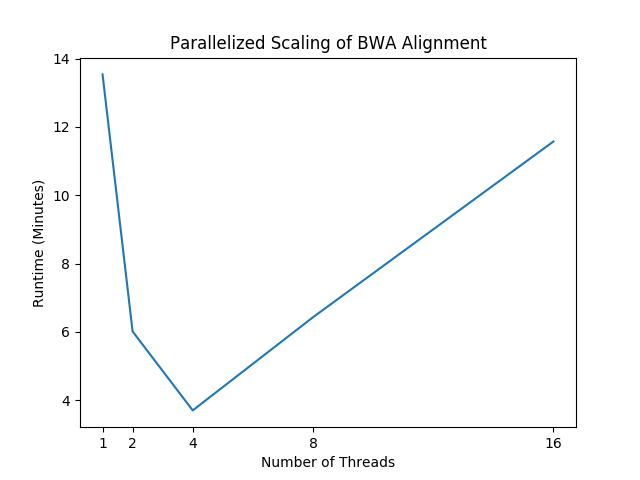
\includegraphics[scale=0.9]{plot_timings.png}
\end{figure}

I hope this helps.\newline

-Jack Hamel

\end{document}
